\documentclass{article}
\usepackage{float}
\usepackage[polish]{babel}
\usepackage[utf8]{inputenc}
\usepackage{polski}
\usepackage{listings} %code environment
\frenchspacing
\setcounter{tocdepth}{2}
\usepackage{graphicx}
\graphicspath{ {images/} }


\begin{document}
	
\begin{titlepage}

\newcommand{\HRule}{\rule{\linewidth}{0.5mm}}

\begin{center}

% university
\textsc{\LARGE Politechnika Warszawska}\\[0.5cm]
\textsc{\Large Wydział Matematyki i Nauk Informacyjnych}\\[1cm]

% logo

\includegraphics[width=2cm, height=2cm]{logo}\\[1cm]


\textsc{\Huge Reprezentacja wiedzy}\\[0.4cm]

%----------------------------------------------------------------------------------------

\HRule \\[0.4cm]
{ \LARGE \bfseries Programy działań z efektami domyślnymi}\\[0.2cm]
 
%----------------------------------------------------------------------------------------

\HRule \\[0.4cm]
{  \bfseries INSTRUKCJA DLA UŻYTKOWNIKA}\\[1.5cm]

% authors
\begin{flushright}
\Large \emph{Autorzy:}\\[0.5cm]
Dragan Łukasz\\
Flis Mateusz\\
Izert Piotr\\
Pielat Mateusz\\
Rząd Przemysław\\
Siry Roman\\
\textbf{Waszkiewicz Piotr}\\
Zawadzka Anna\\[0.9cm]

\end{flushright}

% date
\vfill
{\large 20 czerwca 2016}\\[1cm]
	
\end{center}

\end{titlepage}

\newpage
%----------------------------------------------------------------------------------------
Po uruchomieniu programu widoczne będzie okno pozwalające na zdefiniowanie sygnatury języka (fluenty, akcje i aktorzy):

\begin{figure}[H]
\centering
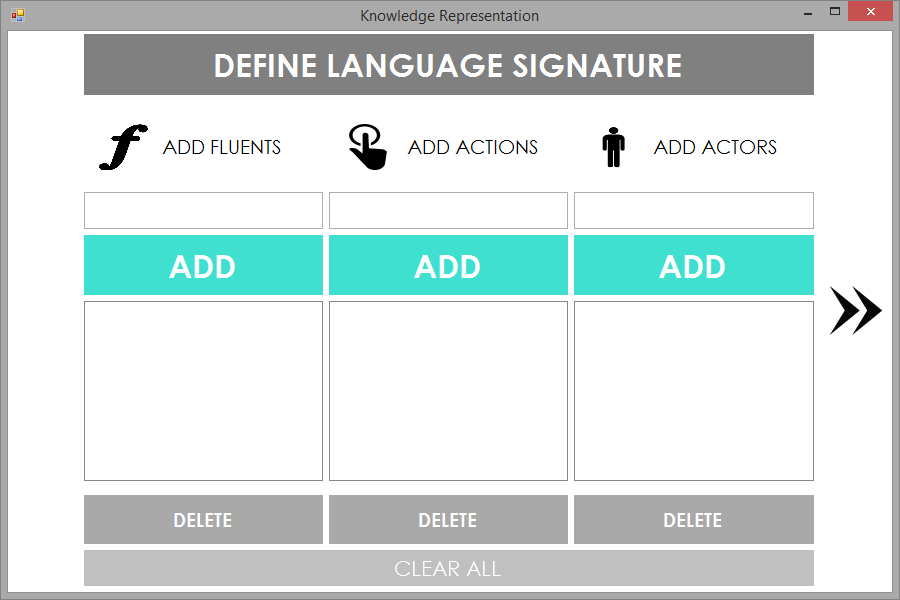
\includegraphics[scale=0.4]{01}
\caption{Okno definiowania sygnatury języka}
\end{figure}


Dodanie nowego elementu odbywa się poprzez wpisanie odpowiedniej nazwy do pola tekstowego i użycie przycisku \textbf{ADD}:

\begin{figure}[H]
\centering
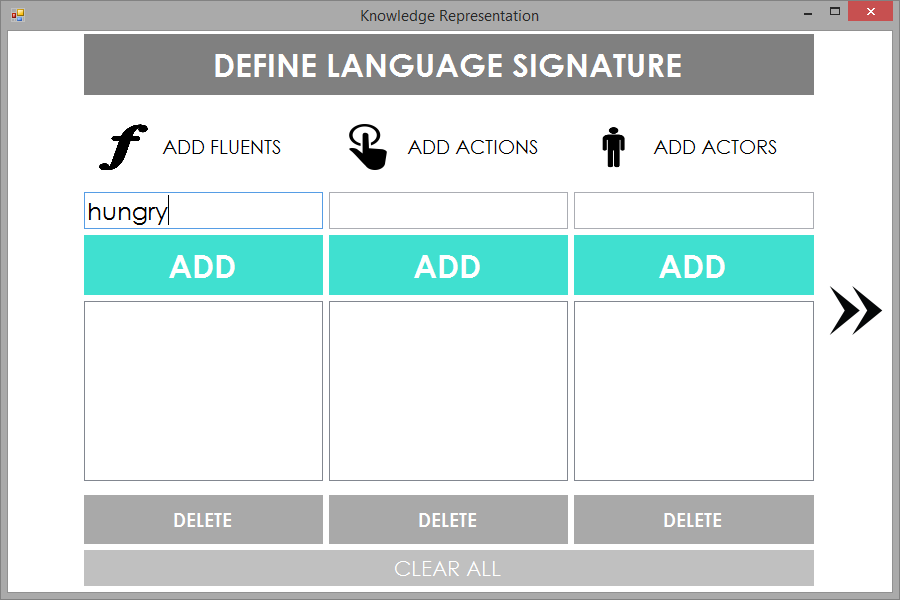
\includegraphics[scale=0.4]{02}
\caption{Okno definiowania sygnatury języka}
\end{figure}
\newpage

Nowy element pojawi się na liście:

\begin{figure}[H]
\centering
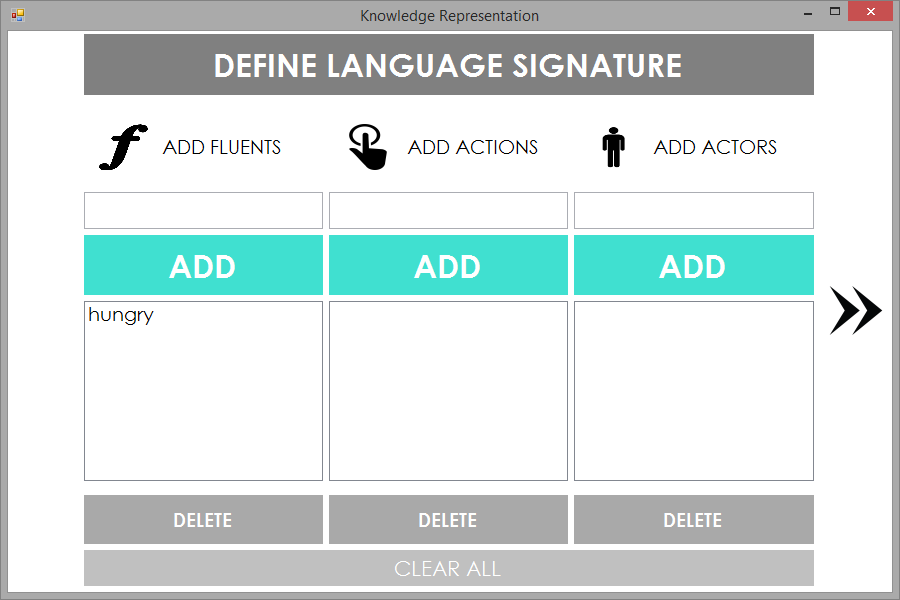
\includegraphics[scale=0.4]{03}
\caption{Okno definiowania sygnatury języka}
\end{figure}

Możliwe jest usunięcie zdefiniowanego obiektu, wystarczy wybrać go z listy i użyć przycisku \textbf{DELETE}:

\begin{figure}[H]
\centering
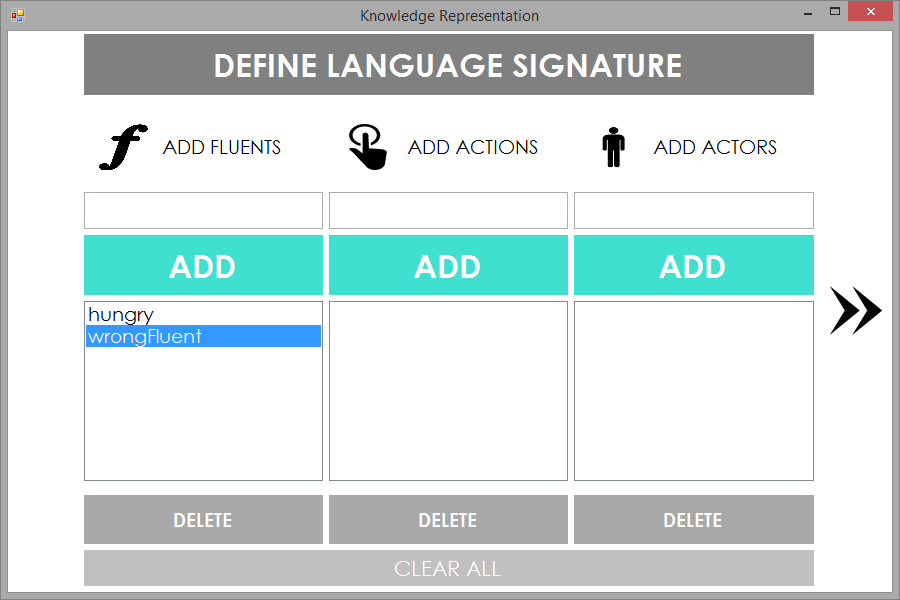
\includegraphics[scale=0.4]{04}
\caption{Okno definiowania sygnatury języka}
\end{figure}

Program umożliwia także usunięcie wszystkich zdefiniowanych elementów na raz przy użyciu przycisku \textbf{CLEAR ALL} na dole okna.
\newpage

Po zdefiniowaniu wszystkich elementów możliwe jest przejście do kolejnego okna klikając strzałkę po prawej stronie okna:

\begin{figure}[H]
\centering
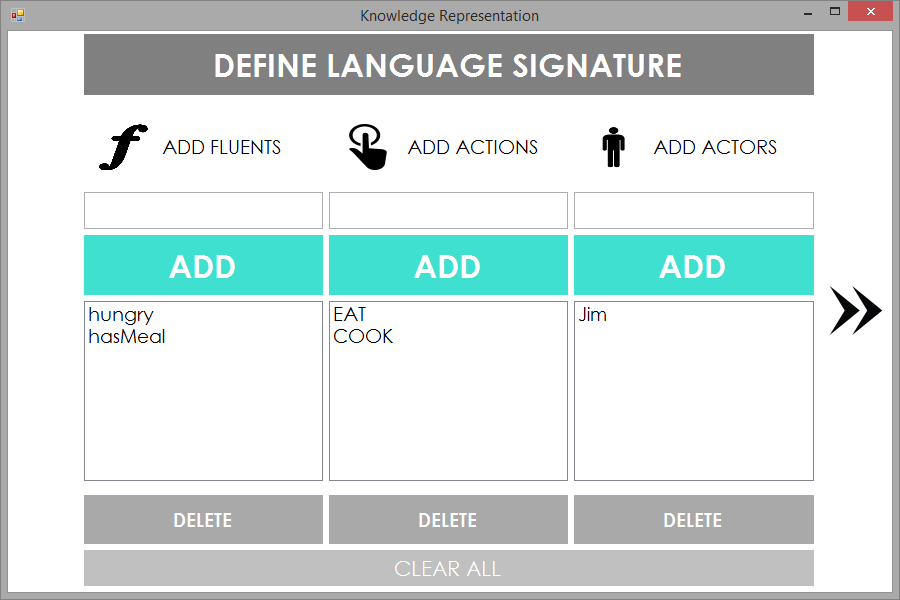
\includegraphics[scale=0.4]{05}
\caption{Okno definiowania sygnatury języka}
\end{figure}

Następnie pojawi się okno definiowania dziedziny. Tutaj możliwe jest dodanie do dziedziny zdań następujących typów: 
\begin{itemize}
\item {\large\texttt{initially $\alpha$}}\\
\item {\large\texttt{$(A,W)$ causes $\alpha$ if $\pi$}}\\
\item {\large\texttt{$(A,W)$ typically causes $\alpha$ if $\pi$}}\\
\item {\large\texttt{$(A,W)$ releases $f$ if $\pi$}}\\
\item {\large\texttt{$(A,W)$ preserves $f$ if $\pi$}}\\
\item {\large\texttt{impossible $(A,W)$ if $\pi$}}\\
\item {\large\texttt{always $\alpha$}}\\
\end{itemize}
gdzie $A$ jest akcją, zaś $W$ jej niepustą listą wykonawców, $f$ fluentem, a $\alpha$ oraz $\pi$ formułami.
\newpage

Przy definiowaniu formuły należy rozpocząć od najbardziej zewnętrznych operacji, możliwe do wyboru to koniunkcja, alternatywa, implikacja, równoważność i negacja, a także wybranie fluentu: 

\begin{figure}[H]
\centering
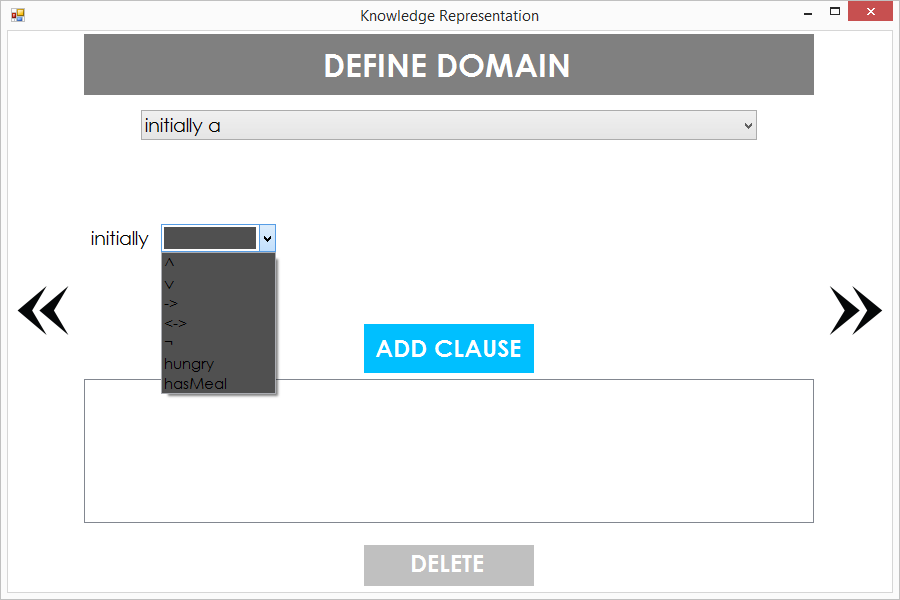
\includegraphics[scale=0.4]{06}
\caption{Okno definiowania dziedziny}
\end{figure}


Przy wyborze spójników logicznych pojawiają się nowe miejsca, w których można definiować poszczególne części formuły:

\begin{figure}[H]
\centering
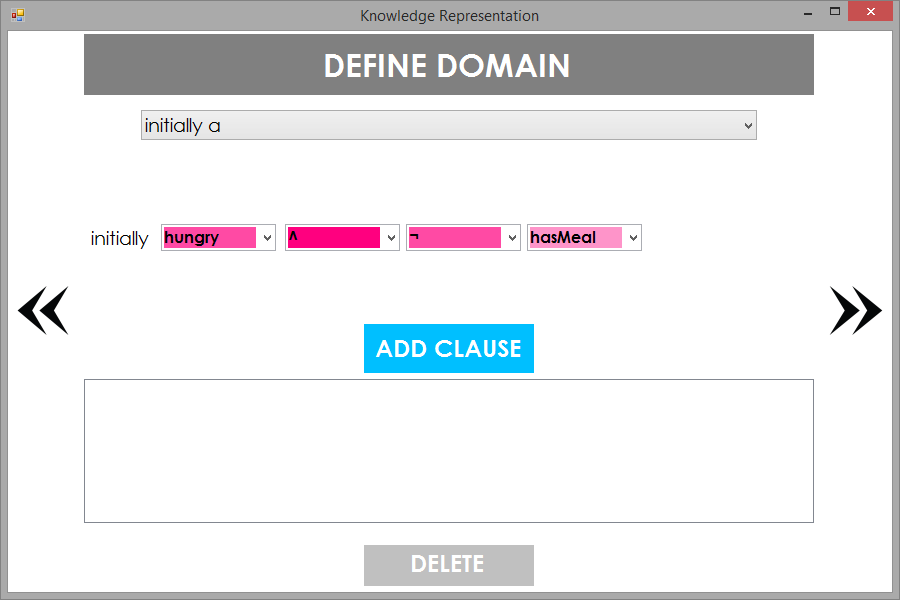
\includegraphics[scale=0.4]{07}
\caption{Okno definiowania dziedziny}
\end{figure}
\newpage

Po zdefiniowaniu odpowiedniego zdania należy użyć przycisku \textbf{ADD CLAUSE} aby dodać nowe zdanie do dziedziny:
 
\begin{figure}[H]
\centering
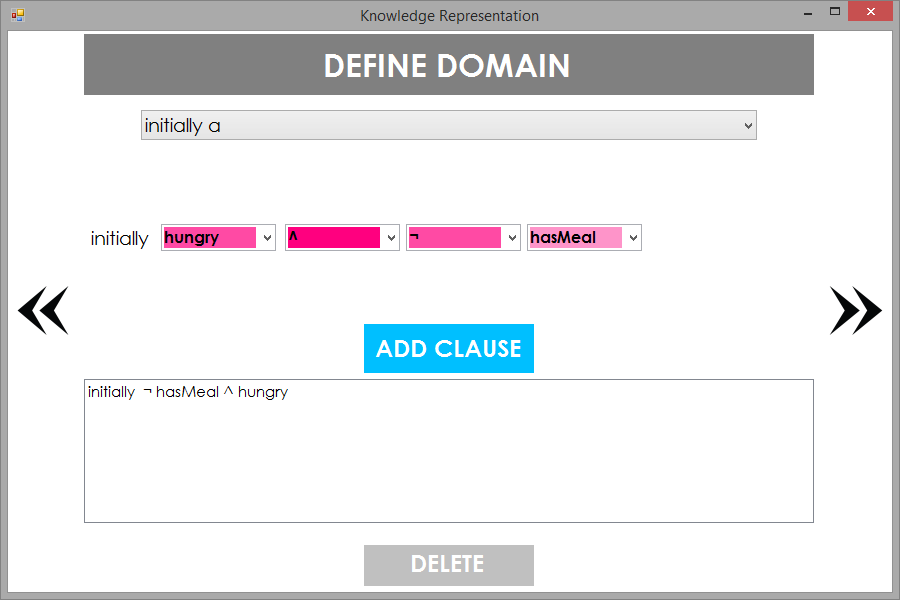
\includegraphics[scale=0.4]{08}
\caption{Okno definiowania dziedziny}
\end{figure}


Możliwe jest usunięcie zdefiniowanego zdania, wystarczy wybrać je z listy i użyć przycisku \textbf{DELETE} na dole okna:

\begin{figure}[H]
\centering
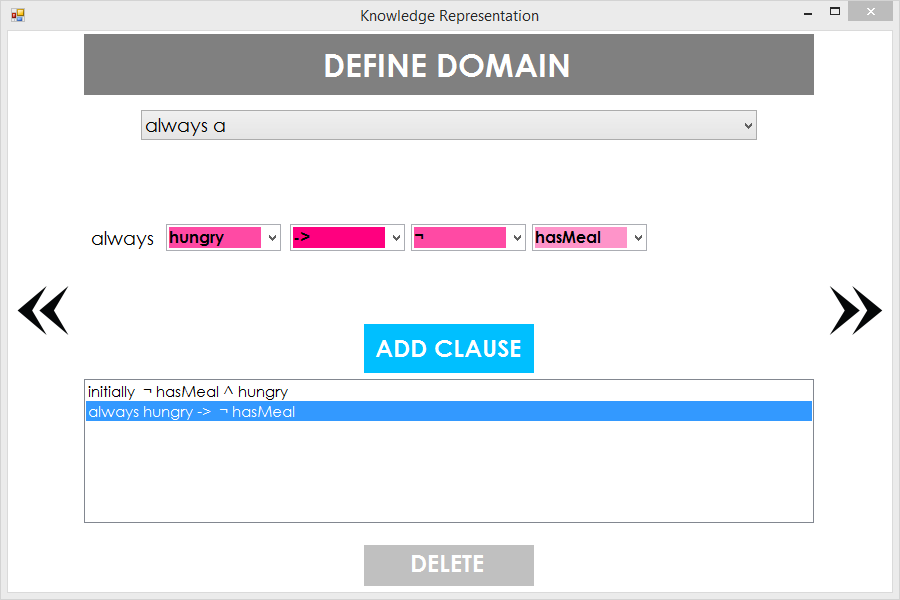
\includegraphics[scale=0.4]{09}
\caption{Okno definiowania dziedziny}
\end{figure}

\newpage
Przy definiowaniu zdań, w których występują wykonawcy, możliwe jest wybranie opcji {\large{$\neg$}}, która oznacza, że akcja jest wykonywana przez wszystkich dostępnych aktorów \textbf{oprócz} tych, którzy zostali zaznaczeni na liście. 

Dodatkowo z listy aktorów możliwe jest wybranie $\epsilon$, co jest równoznaczne z wybraniem wszystkich dostępnych aktorów. 

Po zdefiniowaniu dziedziny można przejść dalej klikając strzałkę w prawą stronę. Z poziomu tego okna możliwy jest również powrót do okna definiowania sygnatury, z tym że wtedy zdefiniowana dziedzina zostaje wyczyszczona (na wypadek jakichkolwiek zmian w sygnaturze języka):

\begin{figure}[H]
\centering
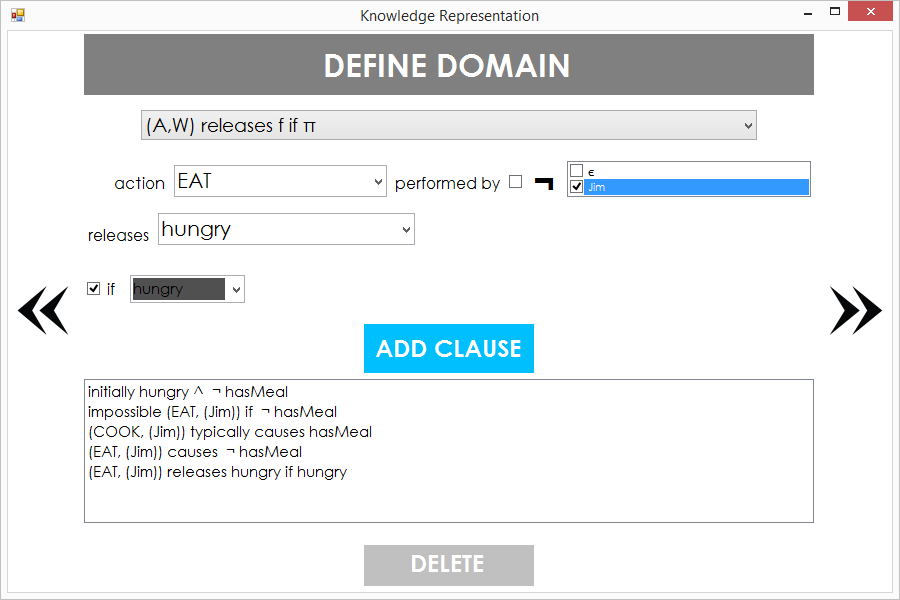
\includegraphics[scale=0.4]{10}
\caption{Okno definiowania dziedziny}
\end{figure}
\newpage

W tym oknie możliwe jest dodanie kolejnych kroków scenariusza:

\begin{figure}[H]
\centering
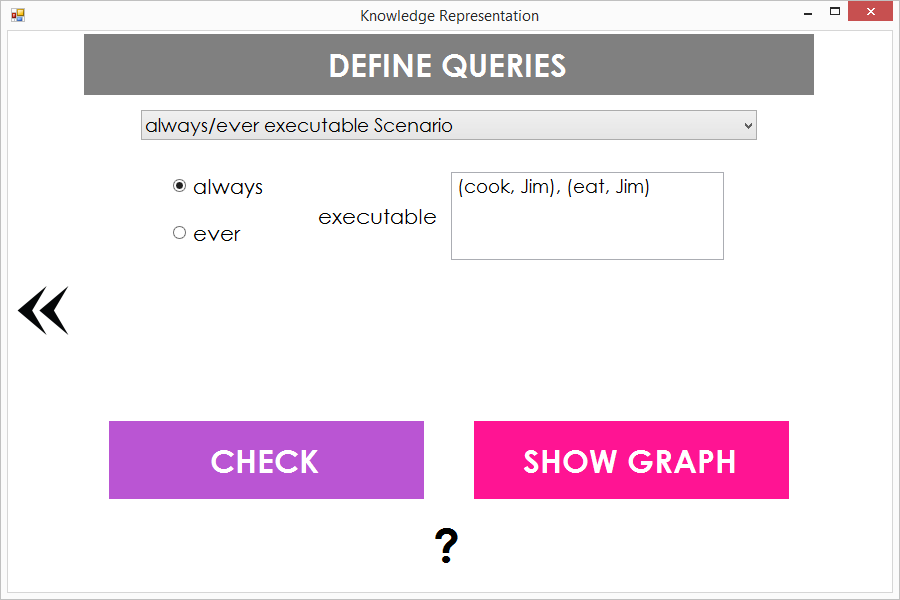
\includegraphics[scale=0.4]{11}
\caption{Okno definiowania scenariusza}
\end{figure}

Kolejnym etapem jest zdefiniowanie zapytań. Możliwe do wyboru to:
\begin{itemize}
\item {\large\texttt{always/ever executable $Scenario$}} \\
Czy podany program działań jest wykonywalny zawsze/kiedykolwiek?
\item {\large\texttt{always/ever/typically accessible $\gamma$ if $\pi$ when $SC$}}\\
Czy wykonanie podanego programu działań z dowolnego stanu spełniającego warunek $\pi$ prowadzi zawsze/kiedykolwiek/na ogół do stanu spełniającego warunek celu $\gamma$ ?
\item {\large\texttt{always/ever/typically accessible $\gamma$ if $\pi$}}\\
Czy z dowolnego stanu spełniającego warunek $\pi$ cel $\gamma$ jest osiągalny zawsze/kiedykolwiek/na ogół?
\item {\large\texttt{always/ever partakes $w$ when $Scenario$}} \\
Czy wskazany wykonawca jest zaangażowany w realizację programu zawsze/kiedykolwiek?
\item {\large\texttt{always/ever/typically $\gamma$ after $SC$ from $\pi$}}\\
Czy po wykonaniu podanego programu działań zawsze/kiedykolwiek/na ogół formuła $\gamma$ jest spełniona w stanie wynikowym?
\end{itemize}





\newpage

\begin{figure}[H]
\centering
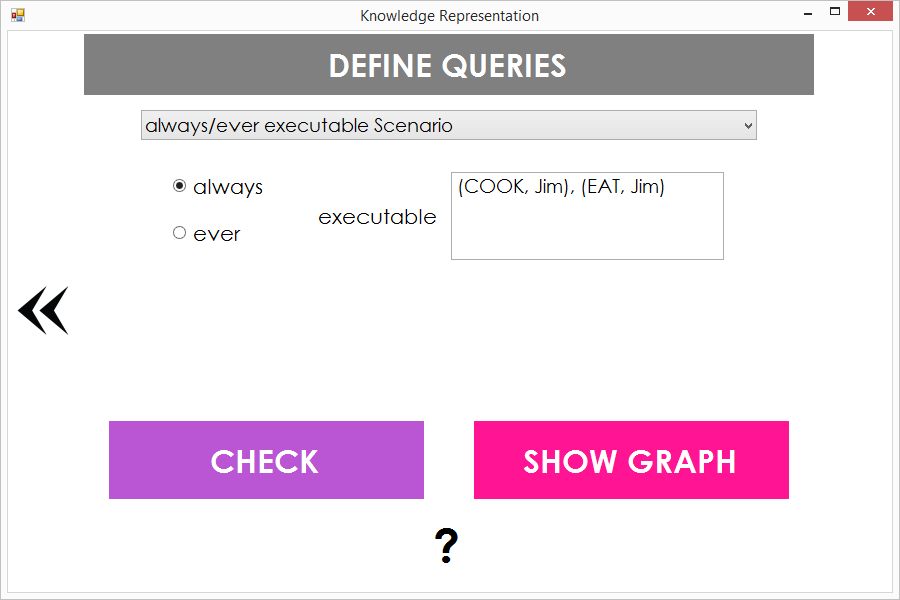
\includegraphics[scale=0.4]{12}
\caption{Okno definiowania kwerend}
\end{figure}


Gdy zapytanie jest zdefiniowane, możliwe jest sprawdzenie odpowiedzi na zadane pytanie poprzez kliknięcie przycisku \textbf{CHECK}. Na dole okna pojawi się odpowiedź ($True/False$):

\begin{figure}[H]
\centering
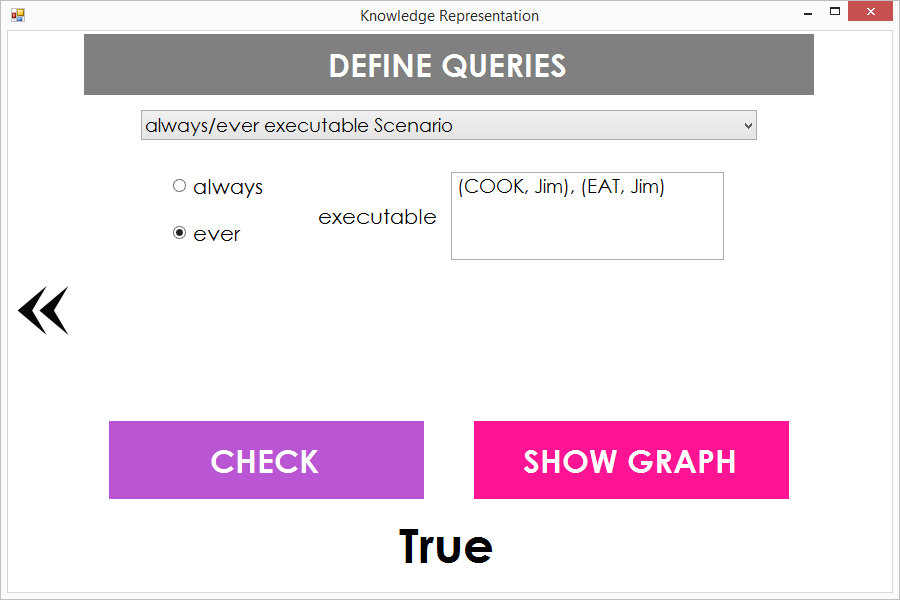
\includegraphics[scale=0.4]{13}
\caption{Okno definiowania kwerend}
\end{figure}

\newpage

Możliwe jest również wyświetlenie grafu zależności poprzez użycie przycisku  \textbf{SHOW GRAPH}:

\begin{figure}[H]
\centering
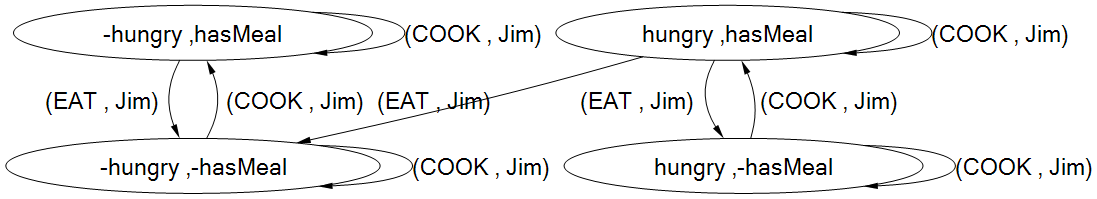
\includegraphics[scale=0.4]{14}
\caption{Graf zależności}
\end{figure}

Na wygenerowanym grafie zaznaczone są możliwe stany początkowe (podwójna linia) oraz krawędzie reprezentujące przejścia typowe i nietypowe, odpowiednio ciagłą i przerywaną linią.

\end{document}
